\documentclass[a4paper,12pt]{article}

% =========================================================
% Packages
% =========================================================

\usepackage[utf8]{inputenc}
\usepackage[T2A]{fontenc}
\usepackage[russian]{babel}

\usepackage{amsmath,amssymb,amsthm}
\usepackage{geometry}
\usepackage{booktabs}
\usepackage{array}
\usepackage{float}
\usepackage{graphicx}
\usepackage{subcaption}
\usepackage{xcolor}
\usepackage{hyperref}

\geometry{
    left=2.5cm,
    right=2cm,
    top=2cm,
    bottom=2cm
}

\hypersetup{
    colorlinks=true,
    linkcolor=blue!60!black,
    urlcolor=blue!60!black,
    citecolor=red!70!black
}

% =========================================================
% Commands
% =========================================================

\newcommand{\R}{\mathbb{R}}
\newcommand{\grad}{\nabla}
\newcommand{\norm}[1]{\left\|#1\right\|}
\newcommand{\eps}{\varepsilon}

% =========================================================
% Title
% =========================================================

\title{
    \textbf{Лабораторная работа №3}\\
    Модификации градиентного спуска
}

\author{
    Георгий Лаврентьев, Дмитрий Коваль\\
    группа М3232
}

\date{Май 2026}

% =========================================================
% Document
% =========================================================

\begin{document}

\maketitle
\vspace{-1em}

% =========================================================
\section{Постановка задачи}
% =========================================================

В работе исследуются модификации градиентного спуска
для задачи безусловной минимизации

\[
f(x)\to\min,
\qquad
f:\R^n\to\R,
\qquad
f\in C^1(\R^n).
\]

Рассматриваются следующие методы:

\begin{enumerate}
    \item Momentum;
    \item Nesterov momentum;
    \item AdaGrad;
    \item RMSProp;
    \item AdaDelta;
    \item Adam.
\end{enumerate}

Исследование проводится на:

\begin{itemize}
    \item хорошо обусловленной квадратичной функции;
    \item плохо обусловленной квадратичной функции;
    \item функции Розенброка;
    \item функции Экли;
    \item функции Химмельблау.
\end{itemize}

Критерием остановки является условие

\[
\norm{\grad f(x_k)} < 10^{-8}.
\]

% =========================================================
\section{Теоретические сведения}
% =========================================================

% =========================================================
\subsection{Общая логика модификаций}
% =========================================================

Большинство современных модификаций градиентного спуска
имеют вид

\[
x_{k+1}=x_k-\alpha_k p_k,
\]

где направление $p_k$ строится не только по текущему
градиенту, но и с использованием внутреннего состояния
метода.

Методы можно разделить на две группы:

\begin{enumerate}
    \item методы с памятью направления:
    Momentum, Nesterov;

    \item адаптивные покоординатные методы:
    AdaGrad, RMSProp, AdaDelta, Adam.
\end{enumerate}

В данной работе рассматривается детерминированная постановка,
то есть используется точный градиент

\[
g_k=\grad f(x_k).
\]

% =========================================================
\subsection{Momentum}
% =========================================================

Метод Momentum задаётся формулами

\[
m_{k+1}=\beta m_k+g_k,
\]

\[
x_{k+1}=x_k-\alpha m_{k+1}.
\]

Параметр $\beta\in[0,1)$ отвечает за силу инерции.

Метод использует сглаженную сумму предыдущих градиентов,
что уменьшает поперечные колебания в узких оврагах.

При слишком больших $\alpha$ и $\beta$
метод может перелетать через минимум,
что приводит к расходимости.

% =========================================================
\subsection{Nesterov}
% =========================================================

Метод Нестерова:

\[
y_k=x_k+\beta(x_k-x_{k-1}),
\]

\[
x_{k+1}=y_k-\alpha \grad f(y_k).
\]

В отличие от Momentum,
градиент вычисляется в предсказанной точке $y_k$.

Это позволяет раньше замечать изменение геометрии функции
и уменьшать излишние колебания траектории.

% =========================================================
\subsection{AdaGrad}
% =========================================================

AdaGrad определяется соотношениями

\[
G_{k+1}=G_k+g_k^2,
\]

\[
x_{k+1}
=
x_k
-
\alpha
\frac{g_k}{\sqrt{G_{k+1}}+\eps}.
\]

Метод автоматически уменьшает шаг
по координатам с большими градиентами.

Главный недостаток AdaGrad —
монотонное накопление $G_k$,
из-за чего шаг со временем стремится к нулю.

% =========================================================
\subsection{RMSProp}
% =========================================================

Метод RMSProp:

\[
G_{k+1}
=
\rho G_k
+
(1-\rho)g_k^2,
\]

\[
x_{k+1}
=
x_k
-
\alpha
\frac{g_k}{\sqrt{G_{k+1}}+\eps}.
\]

В отличие от AdaGrad,
используется экспоненциальное забывание старой информации.

Параметр $\rho$ задаёт длину памяти метода.

% =========================================================
\subsection{AdaDelta}
% =========================================================

AdaDelta определяется формулами

\[
G_{k+1}
=
\rho G_k+(1-\rho)g_k^2,
\]

\[
\Delta x_k
=
-
\frac{\sqrt{u_k+\eps}}
{\sqrt{G_{k+1}+\eps}}
g_k,
\]

\[
u_{k+1}
=
\rho u_k
+
(1-\rho)(\Delta x_k)^2,
\]

\[
x_{k+1}=x_k+\Delta x_k.
\]

В методе одновременно адаптируются:

\begin{itemize}
    \item статистика градиентов;
    \item статистика самих смещений.
\end{itemize}

% =========================================================
\subsection{Adam}
% =========================================================

Метод Adam:

\[
m_{k+1}
=
\beta_1m_k+(1-\beta_1)g_k,
\]

\[
v_{k+1}
=
\beta_2v_k+(1-\beta_2)g_k^2,
\]

\[
\hat m_{k+1}
=
\frac{m_{k+1}}{1-\beta_1^{k+1}},
\]

\[
\hat v_{k+1}
=
\frac{v_{k+1}}{1-\beta_2^{k+1}},
\]

\[
x_{k+1}
=
x_k
-
\alpha
\frac{\hat m_{k+1}}
{\sqrt{\hat v_{k+1}}+\eps}.
\]

Adam сочетает идеи Momentum и RMSProp.

% =========================================================
\section{Тестовые функции}
% =========================================================

% =========================================================
\subsection{Квадратичные функции}
% =========================================================

Хорошо обусловленная функция:

\[
f(x,y)=x^2+y^2.
\]

:contentReference[oaicite:0]{index=0}

Плохо обусловленная функция:

\[
g(x,y)=50x^2+\frac12 y^2.
\]

:contentReference[oaicite:1]{index=1}

% =========================================================
\subsection{Функция Розенброка}
% =========================================================

\[
f(x,y)
=
(1-x)^2+100(y-x^2)^2.
\]

:contentReference[oaicite:2]{index=2}

% =========================================================
\subsection{Функция Экли}
% =========================================================

\[
f(x,y)
=
-20e^{-0.2\sqrt{(x^2+y^2)/2}}
-
e^{(\cos 2\pi x+\cos 2\pi y)/2}
+20+e.
\]

% =========================================================
\subsection{Функция Химмельблау}
% =========================================================

\[
f(x,y)
=
(x^2+y-11)^2+(x+y^2-7)^2.
\]

% =========================================================
\section{Исследование параметров}
% =========================================================

Для каждого метода проводилось исследование зависимости
сходимости от параметров.

Для методов с одним параметром использовались line-графики,
для методов с двумя параметрами --- heatmap.

% =========================================================
\subsection{AdaGrad}
% =========================================================

\begin{figure}[H]
\centering

\begin{subfigure}[b]{0.48\textwidth}
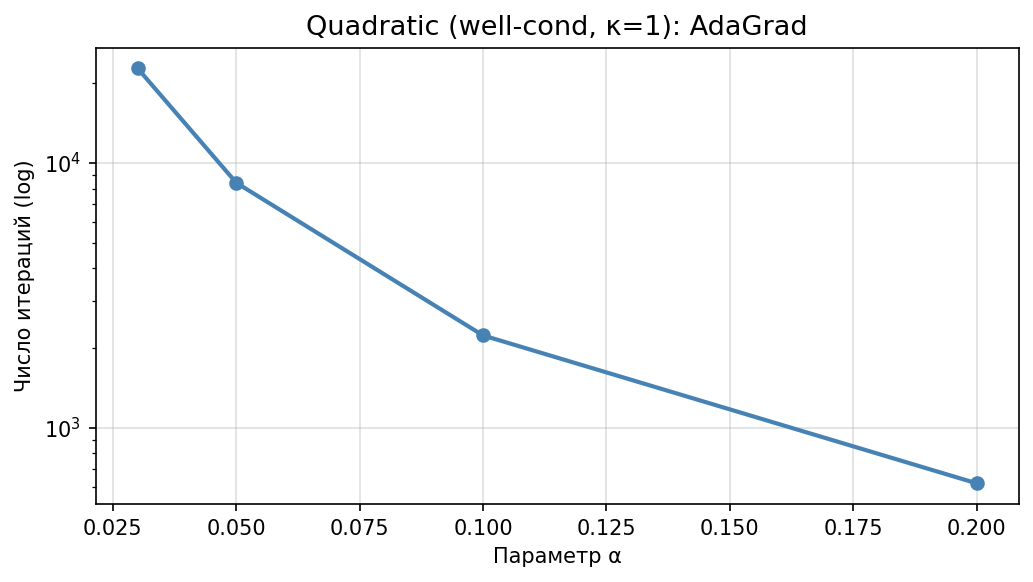
\includegraphics[width=\textwidth]
{results/plots/fig_quad_line_quadratic__well_cond__kappa_1_adagrad_alpha.png}
\caption{$\kappa=1$}
\end{subfigure}
\hfill
\begin{subfigure}[b]{0.48\textwidth}
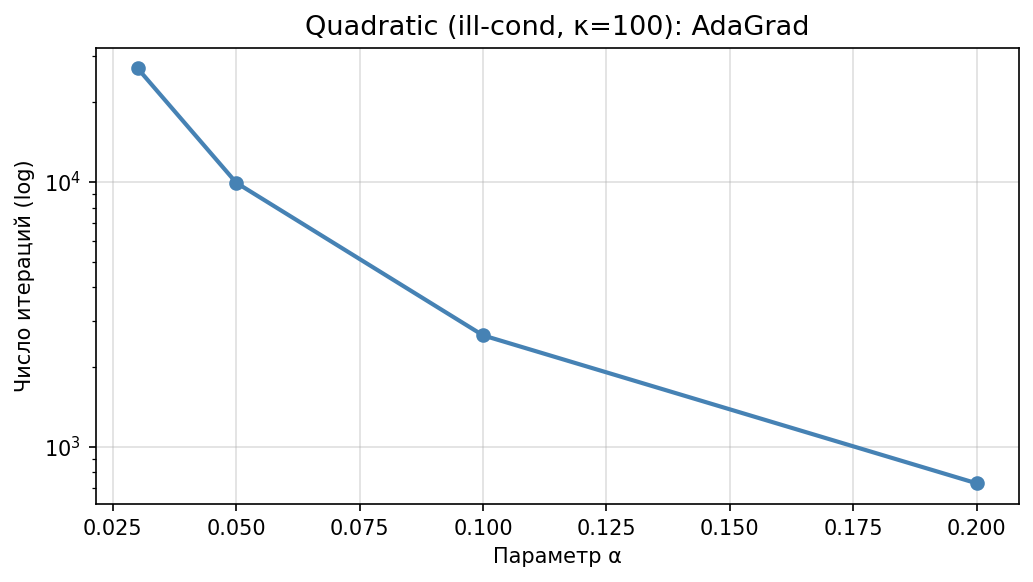
\includegraphics[width=\textwidth]
{results/plots/fig_quad_line_quadratic__ill_cond__kappa_100_adagrad_alpha.png}
\caption{$\kappa=100$}
\end{subfigure}

\caption{AdaGrad: зависимость числа итераций от $\alpha$.}
\end{figure}

На малых $\alpha$ метод сходится медленно,
а на больших $\alpha$ возможны колебания.

Кроме того,
на больших числах итераций наблюдается замедление,
связанное с накоплением величины

\[
G_k=\sum_{t=0}^{k}g_t^2.
\]

Из-за этого эффективный шаг постепенно уменьшается почти до нуля.

% =========================================================
\subsection{Momentum}
% =========================================================

\begin{figure}[H]
\centering

\begin{subfigure}[b]{0.48\textwidth}
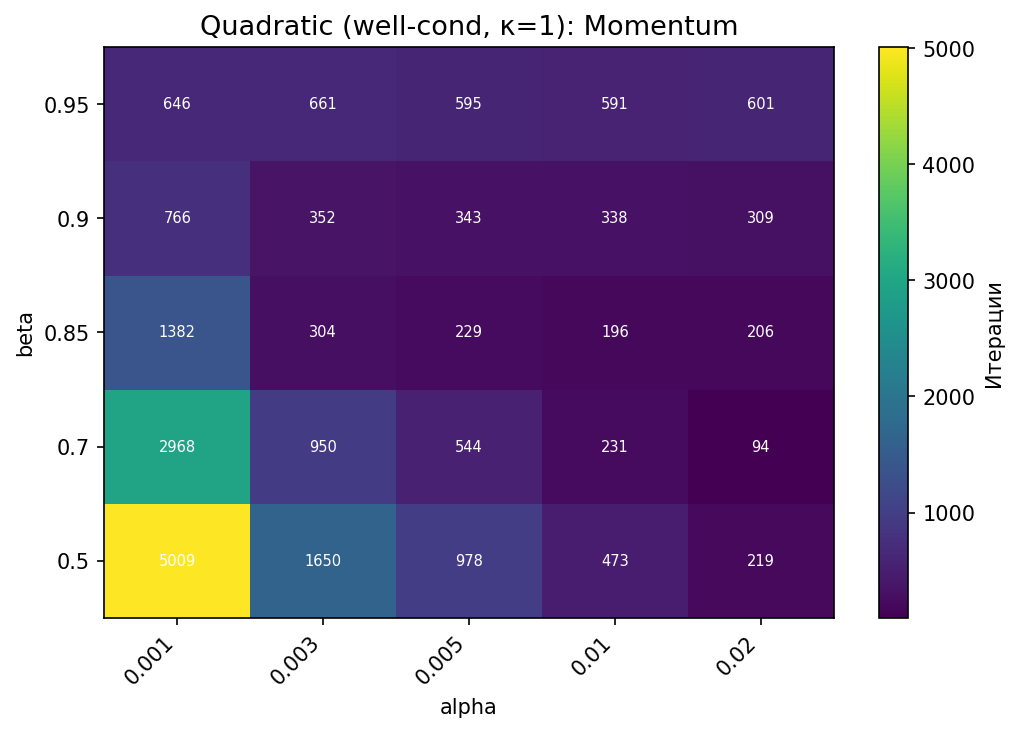
\includegraphics[width=\textwidth]
{results/plots/fig_quad_heat_quadratic__well_cond__kappa_1_momentum_alpha_beta.png}
\caption{$\kappa=1$}
\end{subfigure}
\hfill
\begin{subfigure}[b]{0.48\textwidth}
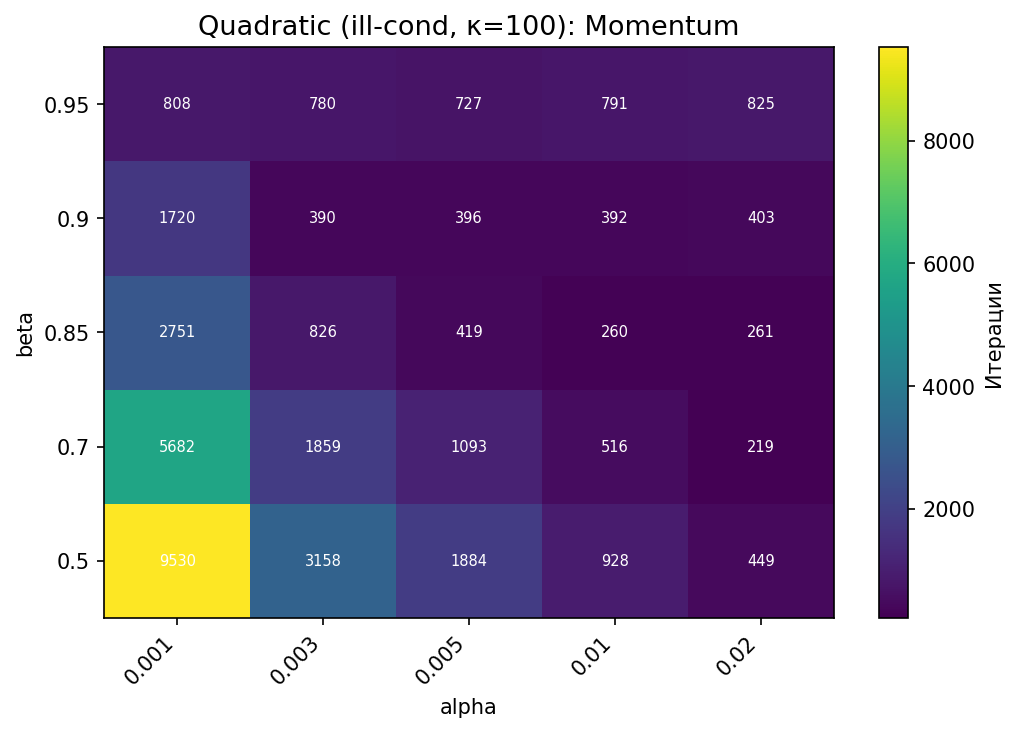
\includegraphics[width=\textwidth]
{results/plots/fig_quad_heat_quadratic__ill_cond__kappa_100_momentum_alpha_beta.png}
\caption{$\kappa=100$}
\end{subfigure}

\caption{Momentum: heatmap по параметрам $(\alpha,\beta)$.}
\end{figure}

При больших значениях $\alpha$ и $\beta$
метод становится неустойчивым.

Инерционный член

\[
\beta(x_k-x_{k-1})
\]

начинает доминировать,
из-за чего траектория перелетает через минимум.

На плохо обусловленной функции это особенно заметно:
траектория начинает колебаться поперёк узкой долины.

% =========================================================
\subsection{Adam}
% =========================================================

\begin{figure}[H]
\centering

\begin{subfigure}[b]{0.48\textwidth}
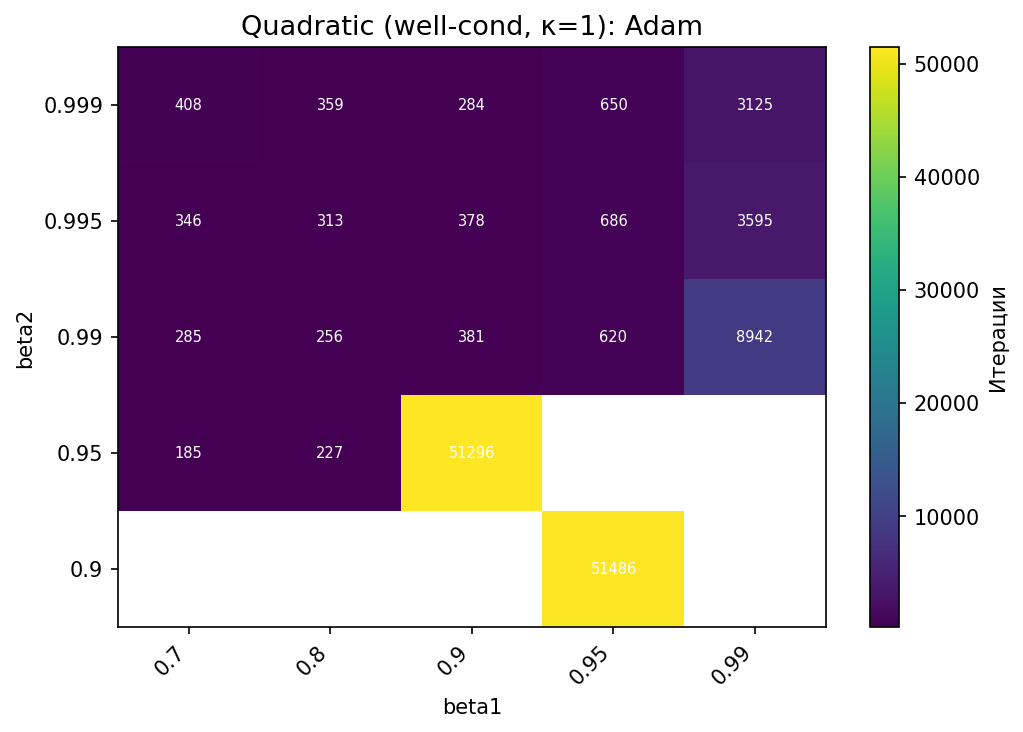
\includegraphics[width=\textwidth]
{results/plots/fig_quad_heat_quadratic__well_cond__kappa_1_adam_beta1_beta2.png}
\caption{$\kappa=1$}
\end{subfigure}
\hfill
\begin{subfigure}[b]{0.48\textwidth}
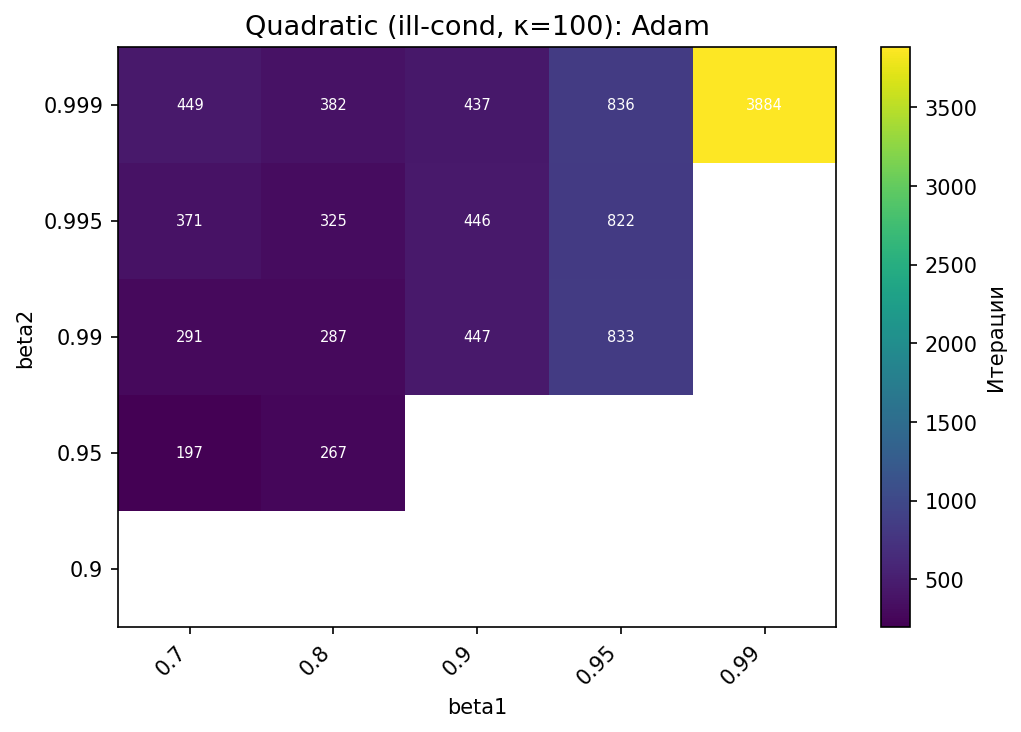
\includegraphics[width=\textwidth]
{results/plots/fig_quad_heat_quadratic__ill_cond__kappa_100_adam_beta1_beta2.png}
\caption{$\kappa=100$}
\end{subfigure}

\caption{Adam: зависимость сходимости от $(\beta_1,\beta_2)$.}
\end{figure}

При слишком больших $\beta_1$ и $\beta_2$
внутренние статистики обновляются слишком медленно.

Метод начинает поздно реагировать
на изменение геометрии функции,
что увеличивает число итераций.

% =========================================================
\section{Траектории методов}
% =========================================================

% =========================================================
\subsection{Квадратичные функции}
% =========================================================

\begin{figure}[H]
\centering

\begin{subfigure}[b]{0.48\textwidth}
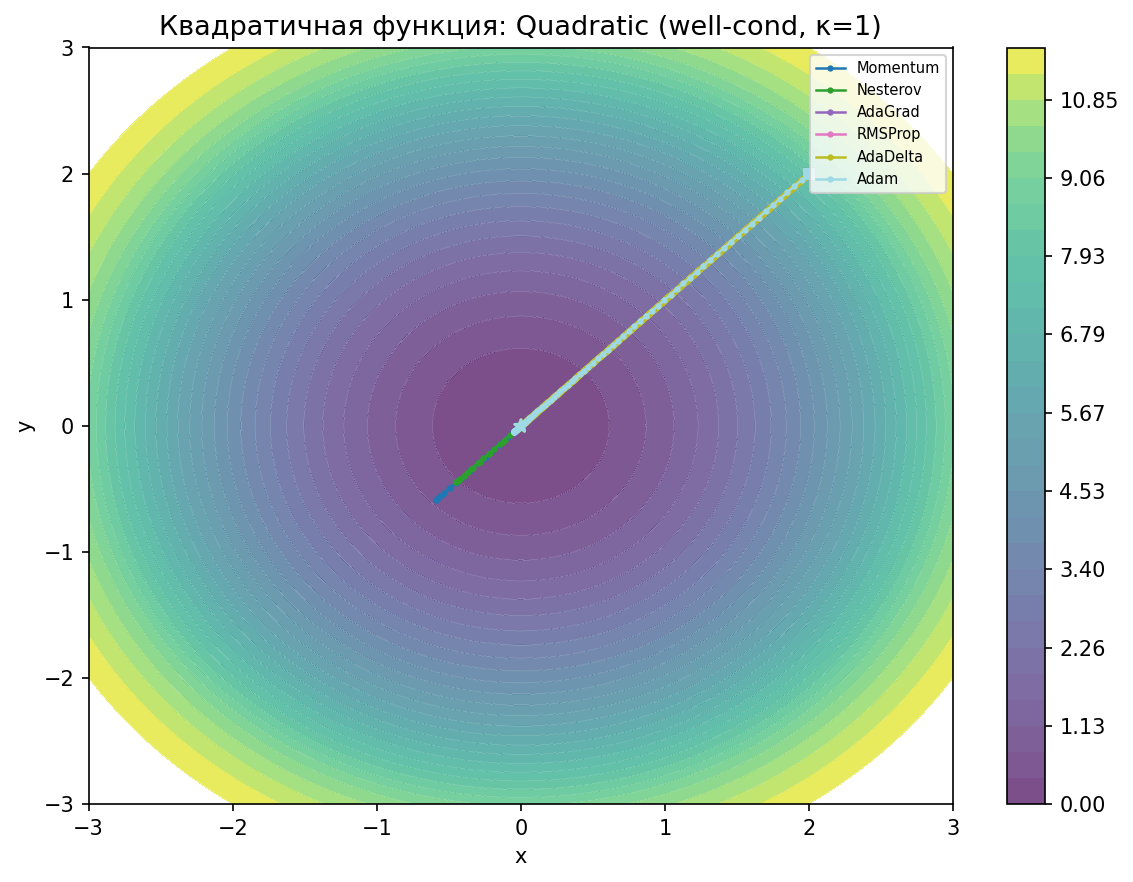
\includegraphics[width=\textwidth]
{results/plots/fig_quad_traj_well.png}
\caption{$\kappa=1$}
\end{subfigure}
\hfill
\begin{subfigure}[b]{0.48\textwidth}
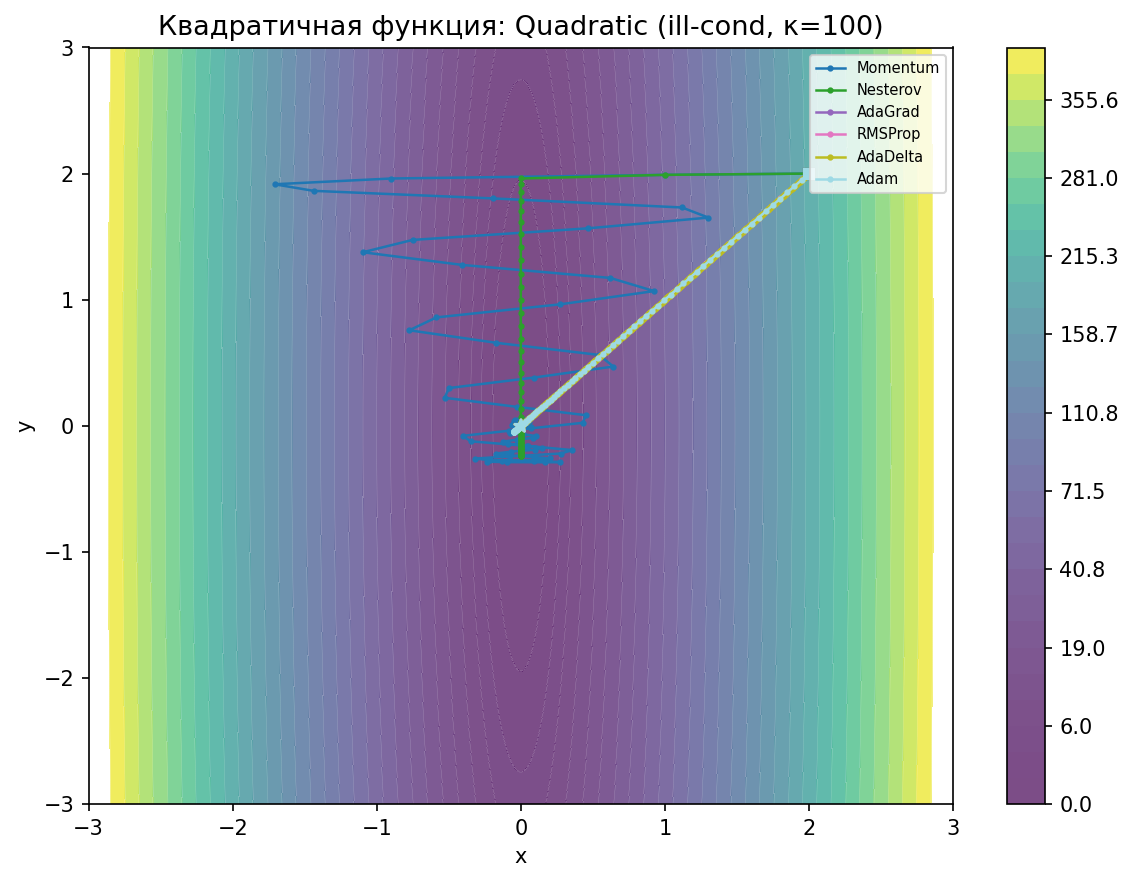
\includegraphics[width=\textwidth]
{results/plots/fig_quad_traj_ill.png}
\caption{$\kappa=100$}
\end{subfigure}

\caption{Траектории методов на квадратичных функциях.}
\end{figure}

На плохо обусловленной квадратичной функции
обычный градиентный спуск и Momentum
демонстрируют выраженные поперечные колебания.

Nesterov корректирует траекторию раньше,
поэтому движение оказывается более устойчивым.

% =========================================================
\subsection{Функция Розенброка}
% =========================================================

\begin{figure}[H]
\centering
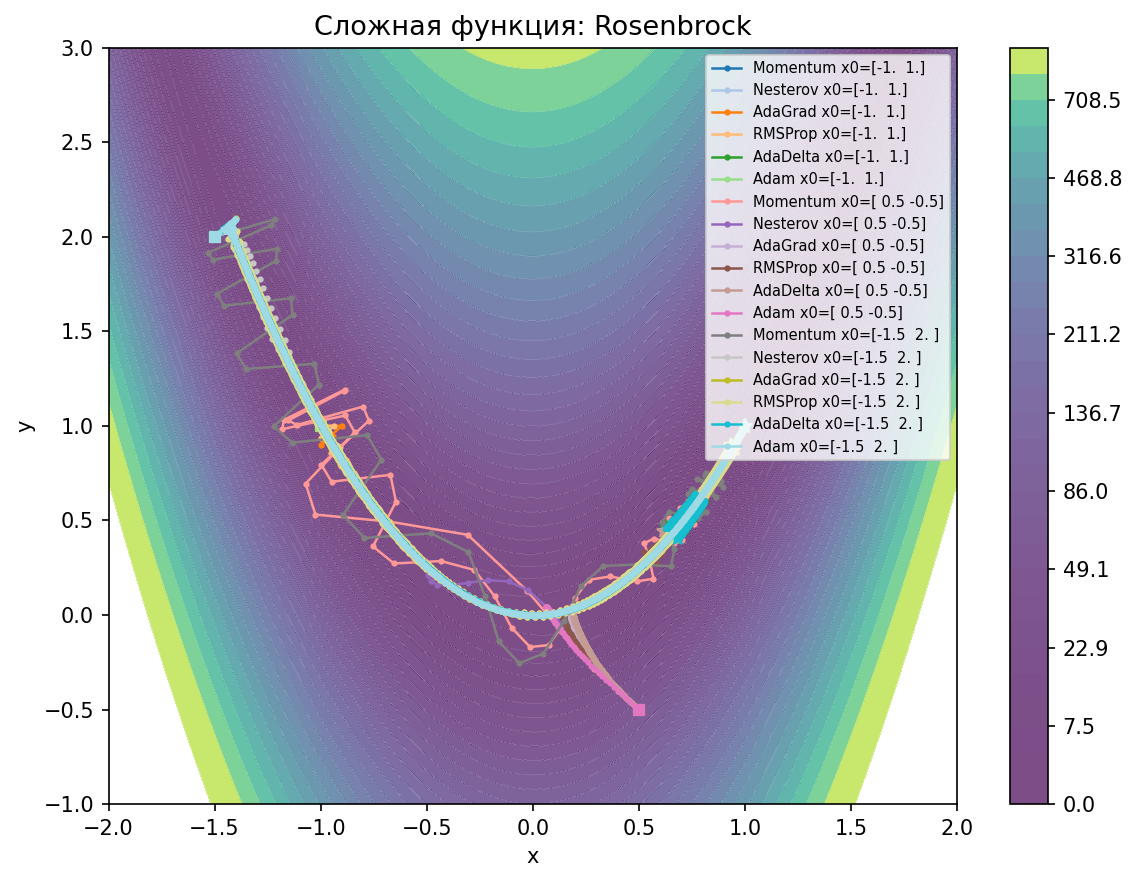
\includegraphics[width=0.8\textwidth]
{results/plots/fig_complex_traj_rosenbrock.png}

\caption{Траектории на функции Розенброка.}
\end{figure}

Функция Розенброка содержит узкий изогнутый овраг.

Из-за этого методы с большим шагом
часто перелетают через дно оврага
и начинают совершать колебания.

Adam и Momentum оказались наиболее устойчивыми.

% =========================================================
\subsection{Функция Экли}
% =========================================================

\begin{figure}[H]
\centering
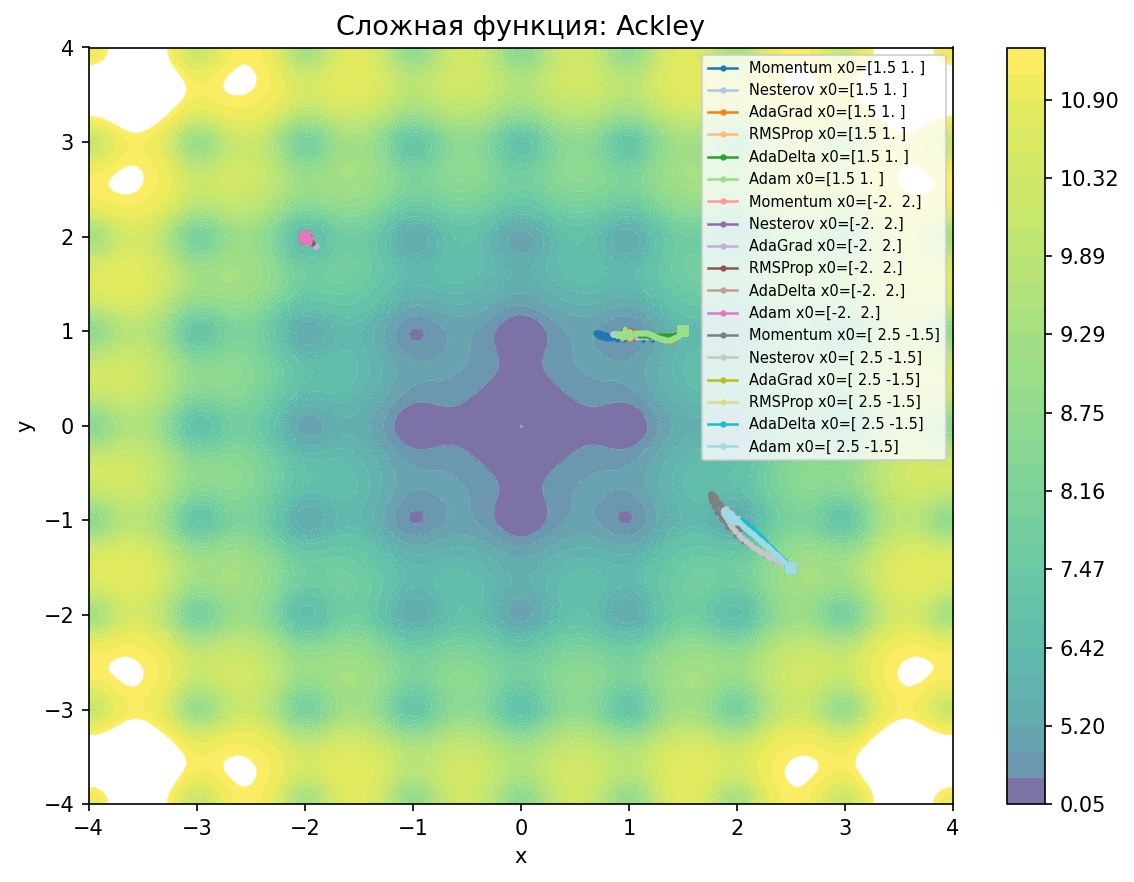
\includegraphics[width=0.8\textwidth]
{results/plots/fig_complex_traj_ackley.png}

\caption{Траектории на функции Экли.}
\end{figure}

Функция Экли имеет большое число локальных минимумов.

Траектория существенно зависит от стартовой точки
и параметров метода.

% =========================================================
\subsection{Функция Химмельблау}
% =========================================================

\begin{figure}[H]
\centering
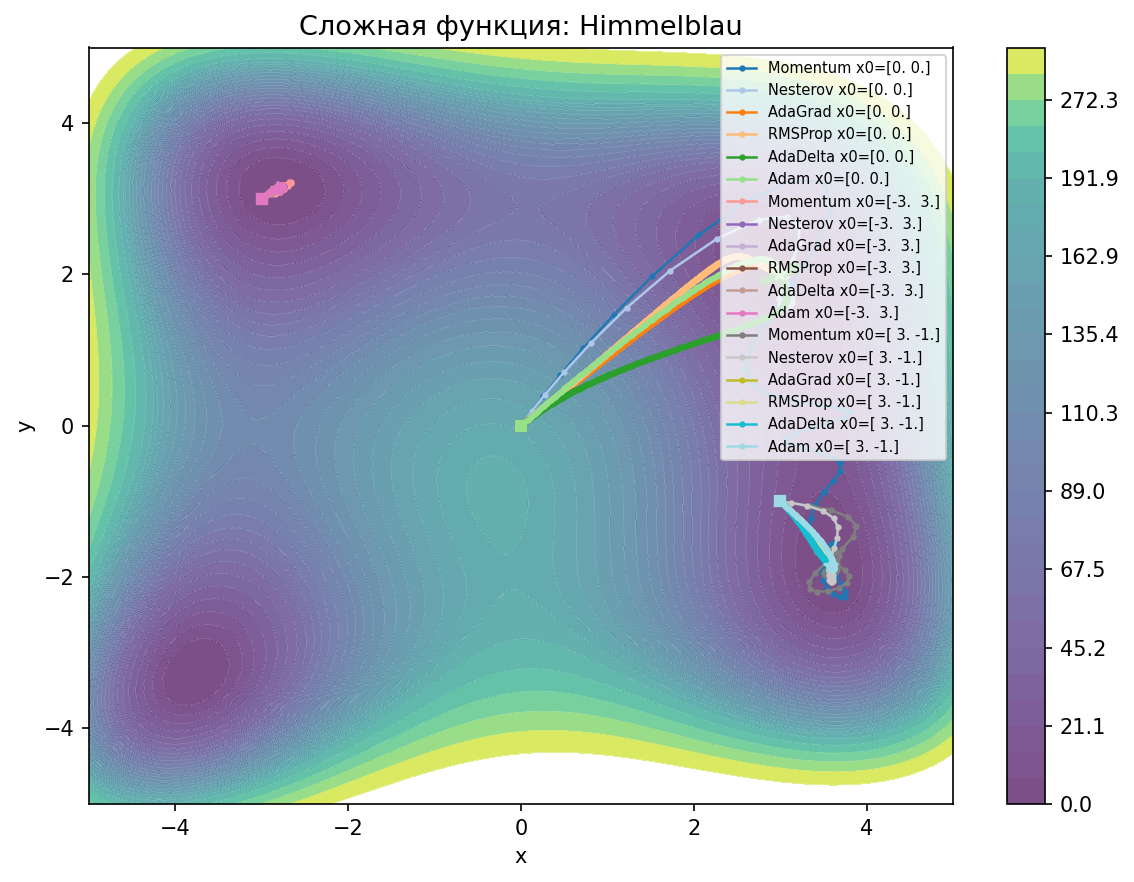
\includegraphics[width=0.8\textwidth]
{results/plots/fig_complex_traj_himmelblau.png}

\caption{Траектории на функции Химмельблау.}
\end{figure}

На функции Химмельблау методы могут сходиться
к различным локальным минимумам.

% =========================================================
\section{Причины расходимости}
% =========================================================

\begin{table}[H]
\centering
\caption{Основные причины неустойчивости методов}
\begin{tabular}{p{3cm} p{10cm}}
\toprule
Метод & Причина расходимости \\
\midrule

Momentum &
слишком сильная инерция и перелёты через минимум \\

Nesterov &
слишком агрессивная экстраполяция \\

AdaGrad &
затухание эффективного шага почти до нуля \\

RMSProp &
нестабильное локальное масштабирование \\

AdaDelta &
сложная динамика адаптации числителя и знаменателя \\

Adam &
слишком медленное обновление статистик при больших $\beta_1,\beta_2$ \\

\bottomrule
\end{tabular}
\end{table}

% =========================================================
\section{Выводы}
% =========================================================

\begin{enumerate}

\item
Momentum и Nesterov уменьшают поперечные колебания
и ускоряют движение вдоль оврагов.

\item
AdaGrad автоматически уменьшает шаг по активным координатам,
но может слишком сильно замедляться.

\item
RMSProp устраняет главный недостаток AdaGrad
за счёт экспоненциального забывания.

\item
AdaDelta дополнительно адаптирует масштаб самих смещений,
что делает динамику метода более сложной.

\item
Adam сочетает идеи Momentum и RMSProp
и в большинстве экспериментов показал наиболее устойчивое поведение.

\item
На плохо обусловленных и многоэкстремальных функциях
результат существенно зависит от параметров метода
и стартовой точки.

\end{enumerate}

\end{document}